\chapter{روش پیشنهادی}
در این فصل روش پیشنهادی و نتایج جدید به‌دست‌آمده در پایان‌نامه توضیح داده می‌شود.
\section{راهکار ما}
تلاش این پروژه برای رسیدن به راهکاری ترکیبی و نوین است. در روش پیشنهاد شده، هم از آزمون منطقی و هم از تحلیل اثرات جانبی استفاده می‌شود. پس این رویکرد را رویکرد ترکیبی می‌نامیم. مزایا و اهداف استفاده از این روش، متشکل از دو موردِ اصلی است: \\
(1) رسیدن به راهکاری که بر طبق استانداردهایی مانند درصد پوشش تروا‌ها(دقت آزمون) و یا تعداد بردار لازم(سرعت آزمون)، نسبتاً بهتر از یا قابل مقایسه با کارهای مرتبط پیشین باشد. \\
(2) به دست آوردن قاعده‌ای برای انتخاب رویکرد بهینه، بین دو رویکرد ذکر شده، با توجه به اندازه‌ی نسبی تروا . 
همان طور که گفته شد، راهکار ترکیبی معرفی شده در این پروژه، از هر دو رویکرد استفاده می‌کند. آزمون منطقی یک مدار الکترونیکی، به طور ساده شده، عبارت است از مشاهده خروجی‌های یک مدار در پاسخ به ورودی‌هایی که خروجی آن‌ها در مدار سالم، از قبل معلوم است. هرگونه مغایرت در خروجی‌ها، به منزله وجود تروا در مدار تفسیر خواهد شد. در این پروژه، آزمون، نه تنها در مرحله آزمون منطقی از بسیاری از روش‌های پیشین کاراتر است، بلکه مهم تر از آن، احتمال موفقیت در مرحله دوم، توسط اندازه‌گیری اثرات جانبی را افزایش می‌دهد. به طور دقیق تر، درمرحله اول، درهنگام تولید بردارهای آزمون منطقی، به جای استفاده از از بردارهای تصادفی، با کمک‌گیری از "ابزار کمکی تروا"، سعی می‌کنیم حدس بزنیم که تروا‌ها در چه گره‌ای از مدار ظاهر خواهند شد. در هنگام آزمون نیز تروا را در نقاطی از مدار قرار می‌دهیم که احتمال حمله به آن‌ها‌‌ بیشتر است. نرم افزار مذکور در حال حاضر طراحی و پیاده‌سازی شده است. توضیح وعملکرد این نرم افزار به بخش 4 واگذار شده است. همچنین از آنجا که نقاط حساس مدار را بدست آورده‌ایم، با الگوریتمی شبیه MERO سعی خواهد شد که فعالیت مدار در نقاط محتمل برای حمله، افزایش داده شود. طراحی و پیاده‌سازی چنین الگوریتمی، یکی از مهم‌ترین چالش‌های پیش روی این پروژه خواهد بود. به طور ساده، خروجی این الگوریتم تعداد محدودی بردار تست، با درصد پوشش بسیار مطلوب و بالا است. بلافاصله توضیحاً علاوه می‌کنیم که کم بودن تعدادِ بردارهای آزمون، یعنی پائین آمدن زمان آزمون. این امر هدف 1 را ارضا خواهد کرد.
در ادامه، لازم است درباره‌ی چگونگی پیاده‌سازی روش اندازه‌گیری اثرات جانبی در این پروژه روشنگری شود. پارامتر مورد تعقیب ما، توان مصرفی خواهد بود. چگونگی این اندازه گیری برای مدارهای سنتز شده، در بخش بعد توضیح داده خواهد شد. اما در این بخش، ارائه یک توضیح منتزع از فرایند اندازه‌گیری توان مصرفی، ضروری به نظر می‌رسد:
در مرحله قبل، مدار را به گونه‌ای تحریک کردیم که فعالیت تروا‌ها بالا رود. حالا که تغییرات همه گره‌ها را محاسبه کرده و در اختیار داریم، اقدام به محاسبه توان مصرفی می‌کنیم. اگر توان مصرفی مدار زیر آزمون، بالاتر از حداکثر توان مصرفی مدار سالم باشد، مدار زیرآزمون، حاوی تروا تشخیص داده می‌شود. 
برای رسیدن به هدف 2، باید دو مرحله ذکر شده را برای تروا‌های کوچک و بزرگ، روی مدارهای مرجع، انجام داد. پس از تکرارهای متعدد، به این جمع‌بندی خواهیم رسید که در مدارهای ترکیبی و ترتیبی --که این مدارها در بخش 4 دقیقاً معرفی شده اند-- اندازه تروا‌‌های مورد بررسی چگونه می‌تواند نوع رویکرد را مشخص کند. به عبارت دیگر، با دسترسی به هدف 2 قادر خواهیم بود که گزارش کنیم: "برای یافتن هر تروا مشخص، در هر مدار مشخص، بهینه است از چه رویکردی استفاده شود."
بدین ترتیب، مفهوم "رویکرد اندازه-آگاه تشخیص تروا"، پیادهسازی خواهد شد.
\section {چالش‌های پیش رو در روش‌های تشخیص تروا}
چالش‌های اصلی روش‌های تشخیص تروا را می‌توان سه چالش عمده دانست:
\begin{itemize}
	\item انتخاب مدل مناسب برای تروا
	\item تولید بردارهای آزمون برای فعالسازی تروا یا افزایش حساسیت به تروا در روش‌های مبتنی بر اثرات جانبی
	\item حذف یا کالیبراسیون نویز اندازه‌گیری، محیط و فرآیند
\end{itemize}
\subsubsection {مدل‌سازی تروا}
پژوهشگران تا کنون مدل‌های متفاوتی برای تروا انتخاب کرده‌اند. برای اعمال یکنواختی در فرآیند و ایجاد امکان مقایسه بین روش‌های مختلف، طبقه بندی سازمان یافته‌ای برای تروا‌ها براساس پارامترهایی که توصیفگر اندازه، میزان مخفی بودن، احتمال فعال شدن، اثر ناشی از تروا و غیره است، ارائه شده‌است. برای مقاصد تولید بردار آزمون، استفاده از مدل تروا با تحریک دیجیتال و اثر دیجیتال، از سایر مدل‌ها مفیدتر است. 
مدل عمومی برای تروا‌های ترکیبی در فصل قبل نشان داده شد. شرط تحریک تروا ترکیبی، رخداد یک مقدار n بیتی در گره‌های داخلی است که فرض شده‌است به اندازه کافی نادر است. خروجی مدار بار گرهی است که وقتی تروا فعال می‌شود، مقدار منطقی‌اش معکوس می‌شود. برای مشکل کردن تشخیص تروا می‌توان از مدل ترتیبی استفاده کرد که برای فعالسازی تروا لازم است این واقعه نادر، چندین بار تکرار شود. در مدل‌های تروا ترتیبی از یک ماشین حالت استفاده می‌شود که در ساده ترین حالت یک شمارنده است. همچنین به جای مدار بار که در شکلها با دروازه XOR مدل شده‌است، هر مدار ترکیبی دیگری می‌تواند قرار گیرد. مدار تحریک نیز که در شکلها به صورت دروازه منطقی AND نمایش داده شده، می‌تواند در حالت کلی هر مدار ترکیبی دیگری باشد.
برای تشخیص تروا با استفاده از روش‌های تحلیل اثرات جانبی، مدل تروا می‌تواند بسیار ساده و در حد یک دروازه منطقی غیرفعال باشد تا اثرش را بر جریان تغذیه سکون مدل کند یا یک خازن باشد تا اثرش را بر تاخیر مسیر مدل کند. با این وجود برای تشخیص تروا با استفاده از نظارت بر جریان گذرا یا تابشهای الکترومغناطیس و غیره، لازم است در مداراتِ تروا فعالیت سوئیچینگ اعمال شود. در این موارد می‌توان از مدل‌های تروای که در روش‌های آزمون منطقی استفاده می‌شوند، استفاده کرد. هرچه اندازه تروا بزرگتر شود، اثرش بر سیگنال‌های جانبی بیشتر می‌شود. از طرفی با افزایش اندازه مدار اصلی، اثر تروا بر این سیگنال‌ها قابل اغماض خواهد بود. بنابراین در مقایسه مدل‌های تروا، اندازه نسبی تروا به مدار اصلی و اثر تروا بر سیگنال‌های جانبی مقایسه می‌شود. 
\subsubsection {تولید بردارهای آزمون}
تولید بردارهای آزمون یکی از مهمترین بخش‌های هر روش تشخیص تروا است. لازم است در طی فرآیند آزمون مدار، هیچ سیگنال فعالساز آزمونی (TE) به طور آشکار موجود نباشد. چرا که مدار تحریک تروا می‌تواند از این سیگنال استفاده کند و با فعال شدن آن، مدار تحریک غیرفعال شود و مانع از تشخیص تروا شود. اعمال بردارهایی که به صورت تصادفی نقاط مختلف مدار را بیازمایند مفید نیست. چرا که تروا‌ها به صورت هوشمندانه درج می‌شوند. بطوریکه سیگنال‌های ورودی تحریک دارای کنترل‌پذیری پایین و سیگنال‌های خروجی بار، دارای مشاهده‌پذیری پایینی باشند. در شکل \ref{fig2-4} انواع مختلف تروا در مدارات ترکیبی و ترتیبی نشان داده شده‌است.
\begin{figure}
	\begin{center}
		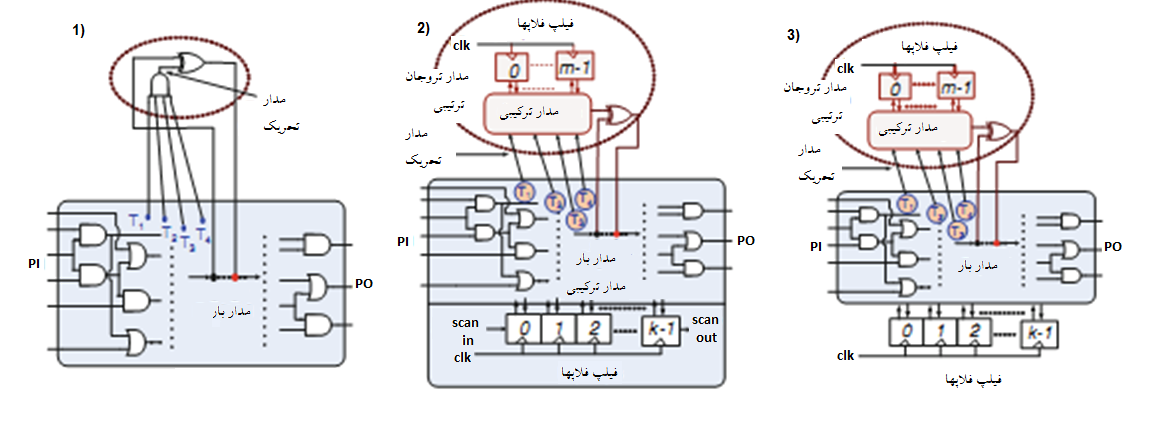
\includegraphics[scale=.5]{figs/fig2-4.png}
		\caption[انواع تروا در مدارهای ترکیبی و ترتیبی]
		{انواع تروا در مدارهای ترکیبی و ترتیبی $\cite{rajendran2011design}$}
		\label{fig2-4}
	\end{center}
\end{figure}
چالش بعدی پیش روی تولید بردارهای آزمون، تعداد بیش از اندازه زیاد تروا‌های ممکن است که با استفاده از مجموعه محدودی از گره‌های داخلی قابل ساخت هستند. با توجه به این موضوع، تولید بردارهای آزمونی که به طور کامل تمام تروا‌های ممکن را تشخیص دهند، از نظر محاسباتی ناممکن است. حتی وقتی گره‌های تحریک را به چهار گره و گره‌های بار را به یک گره محدود کنیم، برای مداری به کوچکی C880 از مجموعه مدارات ISCAS-85 با 451 دروازه منطقی، می‌توان \lr{T≈ 4.1 * 1010} مدار تحریک و \lr{T*(451-4)≈1.8*1013} تروا مختلف داشت. با توجه به مسائل مطرح شده و علل و عوامل دیگری که از حوصله این بحث خارج است، استفاده از روش‌های تولید بردار آزمون آماری $\cite{chakraborty2009mero}$ رایج شده‌است.
\subsubsection {نویز اندازه‌گیری، محیط و فرآیند}
در روش‌های تحلیل اثرات جانبی، تولید بردارهای آزمون به مراتب ساده تر است چرا که نیازی به فعالسازی تروا برای مشاهده نتیجه آن بر پارامتری مثل جریان تغذیه نیست. با این وجود تکنولوژیهای جدید در ابعاد نانو از مشکل تغییرات وسیع در پارامترهای فرآیند رنج می برند. نشان داده شده‌است $\cite{borkar2003parameter}$ که تغییرات فرآیند در تکنولوژی 180 نانومتر تا 30 درصد اختلاف در تاخیر و 20 برابر تغییر در جریان نشتی را موجب می‌شود. شکل 2-4 اثر تغییرات فرآیند را بر ولتاژ آستانه ترانزیستورها نشان می‌دهد که با توزیع گوسی مدل شده‌است. جریان شبیه‌سازی شده همپوشانی زیادی در جریان را نشان می‌دهد که نشانگر اثر مدار تروا است که توسط نویز فرآیند پوشش داده شده‌است. در بخش c شکل، مشاهده می‌شود که تغییرات ناشی از نویز فرآیند تابعی از مقدار پارامتر اندازه‌گیری شده‌است. بنابراین برای مدارات بزرگ با فعالیت سوئیچینگ بالا، جریان تغذیه گذرا می‌تواند تغییرات زیادی داشته باشد که ممکن است اثر تروا‌های کوچک بر جریان را پوشش دهد. بنابراین ممکن است تراشه‌های دارای تروا به عنوان سالم تلقی شوند. 

\begin{figure}
	\begin{center}
		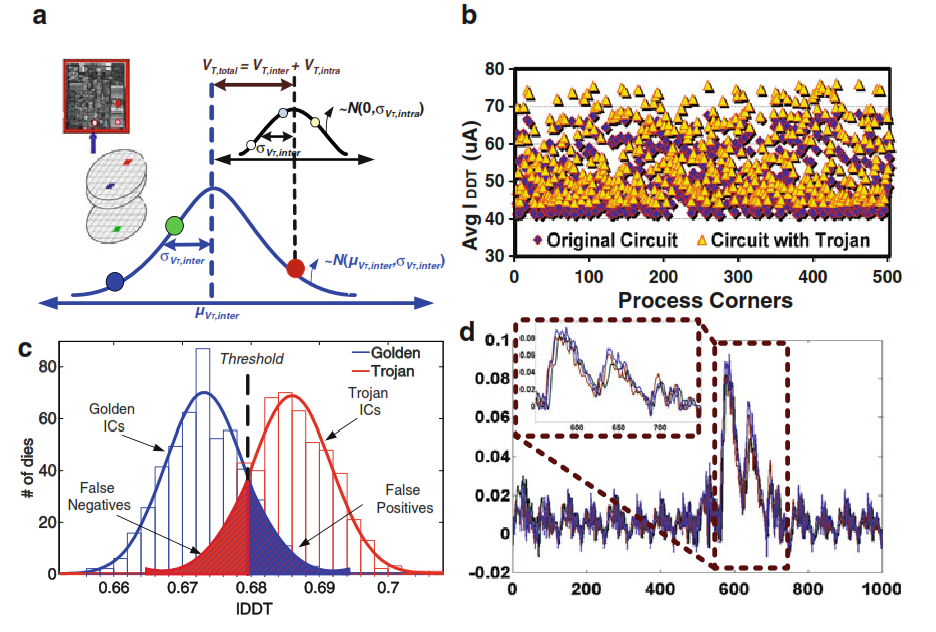
\includegraphics[scale=0.7]{figs/fig3-4.png}
		\caption[اثر تغییر فرآیند بر ولتاژ آستانه و جریان نشتی]
		{اثر تغییر فرآیند بر ولتاژ آستانه و جریان نشتی \cite{borkar2003parameter}}
		\label{fig3-4}
	\end{center}
\end{figure}
یک راه حل، افزایش حساسیت به تروا است. انتخاب بردار ورودی که پارامترهای جانبی در شرایط اعمال آن اندازه‌گیری می‌شوند، نقش مهمی در مقدار اندازه‌گیری شده دارد. بردارها باید به نحوی انتخاب شوند که نقش مدار اصلی کمینه و نقش تروا بیشینه شود. بخش‌بندی به نواحی مختلف و تولید بردار هدایت شده برای القای فعالیت بیشتر در محل‌های محتمل وجود تروا، می‌تواند این امر را میسر کند. از طرف دیگر با کاهش تاثیر نویز فرآیند می‌توان حساسیت روش‌های تشخیص تروا را بالا برد. میانگین گیری آماری از نویز فرآیند و حذف آن از سیگنال اندازه‌گیری شده در پژوهش‌های اخیر $\cite{borkar2003parameter}$ برای افزایش حساسیت انجام شده‌است.

\section{شبیه سازی}
دز این بخش ضمن بررسی روند شبیه‌سازی، نرم افزار‌ها و ابزار مورد استفاده در این پروژه را مرور می‌کنیم.
\subsection{محیط شبیه‌سازی}
در این بخش انواع محیط، ابزار و نرم‌افزارهایی که برای شبیه‌سازی در این پروژه مورد استفاده قرار گرفته می‌شوند را بررسی خواهیم کرد.
\begin{itemize}
	
	\item \subsubsection{\lr{ModelSim}}
	برای آزمون منطقی مدار، و همچنین به دست آوردن میزان فعالیت مدار بر اثر یک دسته بردار آزمون در قالب یک فایل VCD از این محیط شبیه‌سازی بهره می‌بریم. این عمل روی مدار C423 برای این پروژه انجام شد و خروجی آن، ورودی مرحله بعد است. در شکل مقادیر گره‌های این مدار قابل مشاهده است.
	\begin{figure}[H]
		\begin{center}
			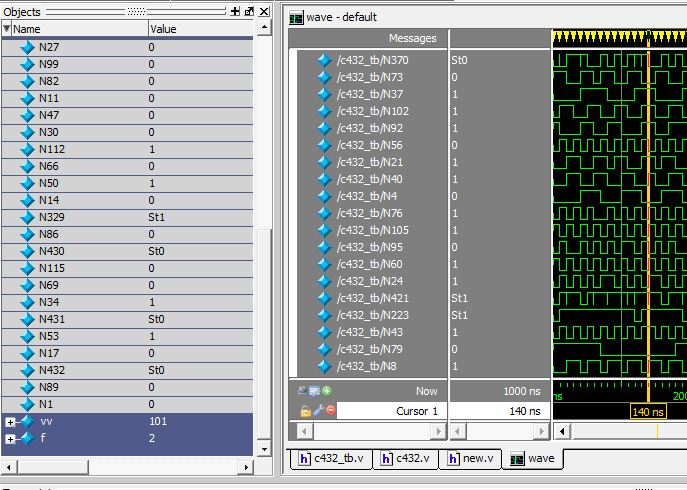
\includegraphics[scale=0.6]{figs/modelsim.jpg}
			\caption{نمای شبیه‌ساز ModelSim} 
			\label{fig1}
		\end{center}
	\end{figure}
	برای آزمون منطقی، از این شبیه‌ساز استفاده می‌کنیم.
	
	
	
	
	\item \subsubsection{\lr{vcd2saif commandline tool}}
	برای محاسبه توان مصرفی، و همچنین پیدا کردن محل قراردادن تروا در مدار، بهتر است فایل فعالیت مدار را به صورت .saif در آوریم. این ابزار عموماً روی سیستم‌های لینوکس که نرم‌افزار 
	\lr{design vision}
	را نصب داشته باشند، پیدا می‌شود.
	خروجی این مرحله، به عنوان ورودی در هر سه مرحله آتی لازم است. این مرحله، در شبیه سازی ویژه این پروژه انجام شد، و خروجی آن به مرحله
	\lr{Trojan Insert Helper}
	داده شد.
	\item \subsubsection{\lr{Synopsis Design Compiler}}
	برای آزمون اثرات جانبی، ابتدا نیاز به مدار سنتز شده داریم. این نرم افزار مدار را برای ما سنتز می‌کند.
	\item \subsubsection{\lr{Synopsis Power Compiler}}
	محاسبه توان مصرفی، از روی یک فایل saif و یک مدار سنتز شده، توسط این ابزار میسر است.
	\item \subsubsection{\lr{Trojan Helper}}
	این نرم افزار، که برای همین پروژه طراحی و پیاده سازی شده است، امکان شناسایی و انتخاب بهترین محل برای قرار دادن تروا در یک مدار را می‌دهد. روش کار بدین صورت است که اطلاعات فایل saif به صورتی تحلیل میشود که گرههای مدار به ترتیب زمان صفر بودن، مدت زمان یک بودن، یا نرخ تغییرات برای کاربر دسته بندی میشوند. فرض اصلی این نرم افزار این است که ترواها معمولا در گره‌های راکد و کم تغییر جایگذاری می‌شوند و در غیر این صورت به راحتی قابل کشف هستند. این نرم افزار از دو ابزار تشکیل شده است:
	(1) بخش سرور - این ابزار یک فایل .saif می‌گیرد، یک Socket برای انتقال اطلاعات به صورت بیسیم، تحت استاندارد  \lr{IEEE 802.11}می‌سازد.
	\begin{figure}
		\begin{center}
			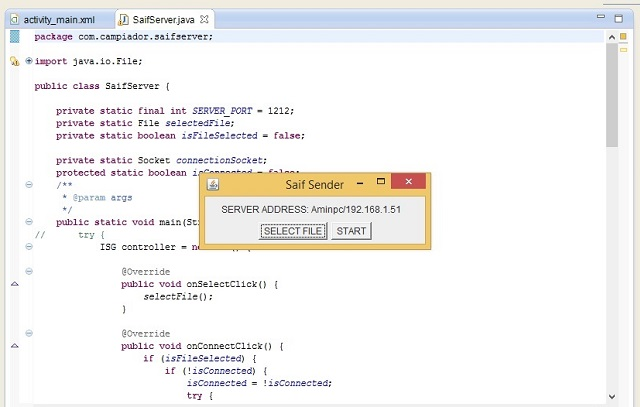
\includegraphics[scale=0.75]{figs/saifServer.jpg}
			\caption{ابزار saif}
			\label{fig2}
		\end{center}
	\end{figure}
	بعد از برقراری ارتباط، این ابزار اقدام به فرستادن اطلاعات فعالیت تک تک گره‌های مدار، تحت پروتکل TCP از روی فایل .saif می‌نماید.
	(2) بخش کلاینت - این بخش هم برای رایانه و هم برای گوشی هوشمند و تبلت پیاده سازی شده است. وظیفه این ابزار، پارس کردن اطلاعات فرستاده شده از طرف سرور، آنالیز و نمایش آن‌ها به گونه‌ایست که کاربر بتواند به راحتی تصمیم بگیرد کدام نقطه برای جایگذاری تروا مناسب‌تر است. برای مثال، در شکل زیر، کاربر درخواست کرده که فهرست گره‌های مدار به ترتیب صعودیِ تعداد سوئیچ‌ها از صفر به یک و برعکس، نمایش داده شود.
	\begin{figure}
		\begin{center}
			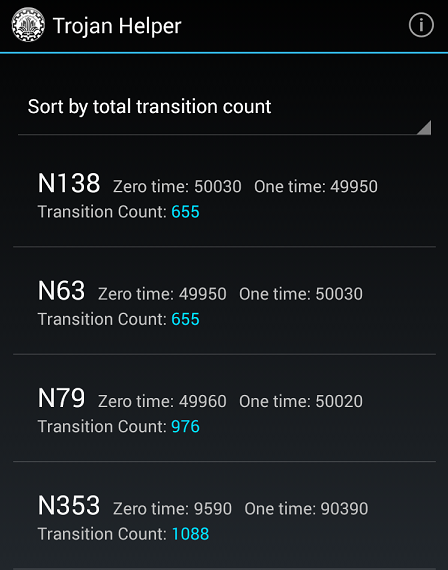
\includegraphics[scale=0.8]{figs/android.png}
			\caption{ابزار saif - مشاهده اطلاعات}
			\label{fig4}
		\end{center}
	\end{figure}
	پس طبق محاسبات انجام شده در مثال بالا، احتمال حضور تروا در گرههای N138 و N63، از باقی گره‌ها بیشتر است. در نتیجه، بهتر است برای شبیه‌سازی یک تروا 2 بیتی برای آزمون، پایه‌های ورودی تروا را از این دو گره بگیریم.
	\item \subsubsection{\lr{Insert Trojan}}
	این برنامه \lr{command-line tool} به زبان جاوا نوشته شده است. هدف این برنامه قرار دادن یک تروا با اندازه مشخص در یک مدار verilog است. طرز استفاده از این دستور بصورت زیر است:
	رو\begin{center}
		
		\lr{java InsertTrojan "../input/c400.v" "4"}
		
	\end{center}
	در این صورت برنامه یک تروا با اندازه 4، در مدار c400 قرار می‌دهد و خروجی را در مدار c400trojan.v ذخیره میکند.
	\item \subsubsection{\lr{Tetramax}}
	
\end{itemize}
از این نرم‌افزار برای حذف بردارهایی که اثر آن‌ها در خروجی قابل مشاهده نیست، استفاده می شود.
\subsection{مجموعه ‌داده}
برای مدارهای میزبان تروا در آزمون‌ها، از مدارهای benchmark ISCAS-85 استفاده شد. 
برای بردارهای ورودی، از حدود 1000 بردار تصادفی با الگوریتمی شبیه الگوریتم MERO طراحی و پیاده‌سازی شد. همان طور که در بخش 3 بیان شد، ویژگی این الگوریتم در آن است که می‌تواند فعالیت مدار را در گره‌های محتمل به حضور تروا، بیشتر کند.
\subsection{نتایج شبیه‌سازی}
در شبیه‌سازی‌ها‌‌ی این پروژه، بستری فرآهم آوردیم تا بتوانیم یک مدار را تحریک و شبیه‌سازی کنیم. در نتیجه تمام ابزار مورد استفاده و چگونگی کار کردن با آن‌ها در طول مراحل شبیه‌سازی برای ما روشن شد. سپس مشخص شد که تنها یک مورد به مجموعه داده‌ها باید اضافه شود. برای تولید این نرم‌افزار، نیاز به طراحی و پیاده‌سازی الگوریتمی مانند MERO داریم که بتواند مجموعه بردارهایی تولید کند که گره‌های تروا‌خیز مدار را بیشتر از حالت عادی تحریک کند.
\section{الگوریتم تولید بردار آزمون} 
این الگوریتم سعی می‌کند به جای استفاده از الگوهای‌های تصادفی، به دنبال مجموعی برداری بگردد که گره‌های تروا‌خیز مدار را تا حد امکان تحریک کنند.
\section{شبیه‌ساز تروا یاب} 
این شبیه‌ساز از الگوریتم بخش قبل استفاده می‌کند، مدار سالم را با بردارهای تولید شده شبیه‌سازی می‌کند و خروجی‌های مدار را برای استفاده ذخیره می‌کند. سپس با استفاده از ابزار درج تروا، مدارهای حاوی تروا تولید می‌کند و سعی می‌کند خروجی‌های مدار را با مدار سالم مقایسه کند. مشاهده اختلاف در خروجی‌ها به معنی کشف تروا است و در صورت وقوع، برنامه به سراغ تروا بعدی می‌رود. در فصل بعد بهبودهایی که بر اثر استفاده از این بردارهای هوشمند به دست آمد، در برابر بردارهای تصادفی مقایسه خواهند شد.
\section{بررسی اثر اندازه تروا بر نتیجه آزمون}
در جدول \ref{tsize} مشاهده می‌شود که با بالا رفتن اندازه مدار، به دلیل گم شدن اثرات جانبی در لابه لای تغییرات فرایند، پیدا کردن مدار تروا سخت تر شد. ولی هرگاه مقدار نسبی مساحت تروا زیاد شد، آزمون اثرات جانبی بهتر جواب داد. این آزمون میانگین نتایج به دست آمده از مدارات ISCAS-85 را نمایش می‌دهد. از سوی دیگر همان طور که با منطق و احتمالات پیش‌بینی می‌شد، آزمون منطقی در پیدا کردن تروا‌های کوچک اکیداً موفق‌تر بوده است.
\begin{table}[t]
	\label{tsize}
	\begin{center}
		\begin{tabular}{| p{4cm} | p{4cm} |p{1cm}|}
			\hline
			\textbf{ آزمون اثرات جانبی} & \textbf{ آزمون منطقی} & \textbf{اندازه تروجان}\\ \hline \hline
			78 & 97 &\textbf{2} \\ \hline
			82 & 95 &\textbf{4} \\ \hline
			86 & 94 &\textbf{8} \\ \hline
			87 & 93 &\textbf{12} \\ \hline
			92 & 76 &\textbf{16} \\ \hline
		\end{tabular}
		\caption{
			اثر اندازه تروا بر نتیجه آزمون (نرخ کشف تروا)}
		
	\end{center}
\end{table}

\section{مقایسه نرخ کشف آزمون اثرات جانبی با استفاده از بردارهای هوشمند و تصادفی}
\begin{table}[t]
	\label{tsideivectors}
	\begin{center}
		\begin{tabular}{| p{4cm} | p{4cm} |p{2cm}|}
			\hline
			\textbf{ بردار تصادفی} & \textbf{ بردار هوشمند} & \textbf{مدل مدار} \\ \hline \hline
			99 & 99 &\textbf{c432} \\ \hline
			98 & 98 &\textbf{c499} \\ \hline
			98 & 98 &\textbf{c880} \\ \hline
			94 & 97 &\textbf{c1355} \\ \hline
			95 & 98 &\textbf{c1908} \\ \hline
			88 & 96 &\textbf{c2670} \\ \hline
			86 & 93 &\textbf{c3540} \\ \hline
			83 & 92 &\textbf{c5315} \\ \hline
			80 & 92 &\textbf{c6288} \\ \hline
			77 & 86 &\textbf{c7552} \\ \hline 
		\end{tabular}
		\caption{
		مقایسه آزمون اثرات جانبی با بردارهای هوشمند و تصادفی(نرخ کشف تروا)}
	\end{center}
\end{table}
همان طور که در جدول \ref{tsideivectors} مشاهده می‌شود بردارهای هوشمند ما بسیار بهتر از بردارهای تصادفی تروا‌ها را کشف می‌کنند. دلیل آن است که بیشتر توان مصرفی در سلول‌های
\lr{TSMC 130 nm}
متشکل از توان پویا می‌باشد. این توان پویا وابسته به میزان سوئیچینگ گره‌های مدار است. حال که ما مدار را ثابت نگه داشته و بیشتر سعی بر فعال کردن گره‌های تروا‌خیز داشتیم، این اختلاف به خوبی در توان مصرفی خود را نشان داد. نکته دیگری که به نظر می‌رسد این است که با بزرگ شدن هرچه بیشتر مدار میزبان، روش هوشمند ما ارزش خود را بیشتر نشان می‌دهد.





